\documentclass[12pt,a4paper]{article}

% ── Paquetes ────────────────────────────────────────────────
\usepackage[utf8]{inputenc}
\usepackage[T1]{fontenc}
\usepackage{amsmath, amssymb, amsfonts, amsthm}
\usepackage{mathtools}
\usepackage{graphicx}
\usepackage{geometry}
\usepackage{algorithm}
\usepackage{algorithmic}
\usepackage{tikz}
\usepackage{pgfplots}
\pgfplotsset{compat=1.18}
\usetikzlibrary{shapes.geometric, arrows.meta, positioning,
                decorations.pathreplacing, fit, backgrounds,
                calc, patterns}
\usepackage{xcolor}
\usepackage{booktabs}
\usepackage{multirow}
\usepackage{hyperref}
\hypersetup{colorlinks=true, linkcolor=blue, citecolor=blue, urlcolor=blue}

% ── Márgenes ────────────────────────────────────────────────
\geometry{margin=1in}

% ── Colores ─────────────────────────────────────────────────
\definecolor{col1}{RGB}{52,101,164}
\definecolor{col2}{RGB}{56,142,60}
\definecolor{col3}{RGB}{230,119,0}
\definecolor{col4}{RGB}{198,40,40}
\definecolor{col5}{RGB}{103,58,183}
\definecolor{coldark}{RGB}{40,40,60}
\definecolor{collight}{RGB}{240,244,255}

% ── Teoremas ────────────────────────────────────────────────
\newtheorem{definition}{Definition}
\newtheorem{proposition}{Proposition}
\newtheorem{remark}{Remark}

% ── Operadores ──────────────────────────────────────────────
\DeclareMathOperator{\diag}{diag}
\DeclareMathOperator{\softmax}{softmax}
\newcommand{\tens}[1]{\boldsymbol{\mathcal{#1}}}
\newcommand{\R}{\mathbb{R}}
\newcommand{\E}{\mathbb{E}}

% ── Título ──────────────────────────────────────────────────
\title{\textbf{Agentic Theory III: Stimulus Tensor Propagation,\\
Emergent High-Order Addictions, and the Tensorial\\
Output Stream in Agentic Neural Networks}}
\author{Justo Tapiador García \\
Department of Artificial Intelligence and Neuroscience \\
Universidad de Alicante (UA)}
\date{\today}

% ════════════════════════════════════════════════════════════
%% ── MARCA DE AGUA WALLERMAX-AI ──────────────────────────────────────────────
%% Generado automáticamente por add_watermark.js
%% Requiere: eso-pic, rotating, xcolor, calc  (incluidos en TeX Live / MiKTeX)
\usepackage{eso-pic}       % AddToShipoutPictureBG
\usepackage{rotating}      % sideways / rotatebox
\usepackage{xcolor}        % colores
\usepackage{calc}          % \paperheight, arithmetic

\AddToShipoutPictureBG{%
  \AtPageLowerLeft{%
    % Posición: 1.05 cm desde el borde izquierdo,
    % centrado verticalmente (paperheight/2)
    \put(\LenToUnit{1.05cm}, \LenToUnit{0.5\paperheight}){%
      \rotatebox{90}{%
        \color{red!23!white}%
        \Large%
        \sffamily\bfseries
        WALLERMAX-AI 2604.00014\quad\textbullet\quad24/04/2026%
      }%
    }%
  }%
}
%% ────────────────────────────────────────────────────────────────────────────


\begin{document}
% ════════════════════════════════════════════════════════════

\maketitle

\begin{abstract}
The two preceding papers in this series introduced the Artificial Junky Neuron (AJN)
as an atomic agentic unit and established its composition into multi-layer Agentic
Neural Networks (ANN-$\Psi$). The present work addresses two phenomena that emerge
specifically from the network topology and cannot be observed at the single-unit level.

First, we formalize the \textit{transformation and generalization of stimulus tensors
across layers}: a low-level sensory tensor received by the first layer undergoes
successive recodings---abstraction, fusion, and re-projection---as it propagates
upward through an ANN-$\Psi$. Each AJN layer constructs a new, higher-dimensional
stimulus tensor from the praxic outputs of the layer below, creating a stimulus
hierarchy. We show that this hierarchy supports the emergence of \textit{high-order
addictions}: stable craving attractors at intermediate and deep layers that are not
present in the original sensory signal but arise from the network's own internal
dynamics. High-order addictions are defined formally, and their conditions of
existence are derived.

Second, we argue that the output of an ANN-$\Psi$ is not, in general, a single
tensor event but a \textit{tensorial praxic stream} (TPS): a temporally extended,
causally interleaved sequence of partial praxis tensors, each followed by
environmental feedback before the next is emitted. We formalize the TPS as a
stochastic process, derive the closed-loop dynamics it induces over the
environment's state space, and show that classical single-shot output is a
degenerate limiting case of the TPS. The combination of hierarchical stimulus
generalization and streaming praxic output defines a new computational paradigm
we term \textit{Deep Agentic Flow} (DAF).
\end{abstract}

\tableofcontents
\newpage

% ════════════════════════════════════════════════════════════
\section{Introduction}
% ════════════════════════════════════════════════════════════

A single Artificial Junky Neuron (AJN) interacts with the world through the
simplest possible sensorimotor loop: it receives a stimulus tensor $\tens{S}_t$,
evaluates its intensity $\alpha_t$, emits a praxis $\tens{P}_t$ via transducers,
and observes the perturbed stimulus $\tens{S}_{t+1}$. The loop is tight, local,
and concrete.

When AJN units are organized into layers and layers are stacked into an
ANN-$\Psi$~\cite{tapiador2024annpsi}, two qualitatively new phenomena arise that
deserve dedicated analysis.

\paragraph{Stimulus propagation and abstraction.}
The stimulus entering layer $\ell+1$ is not the raw environmental tensor
$\tens{S}_t^{(0)}$ but a \textit{derived} tensor---the aggregate praxic output
of layer $\ell$, processed by an intermediate transducer. This derived tensor
carries information about layer $\ell$'s motivational state, not merely the raw
sensory signal. As this process repeats across $L$ layers, the stimulus undergoes
a succession of transformations that progressively abstract, compress, and
recombine the original sensory content. Deep layers ``see'' a stimulus that is
the emergent product of all preceding layers' agentic activities. We show that
this process creates conditions for \textit{high-order addictions}: craving
attractors that are constituted not by any single feature of the external world
but by relational patterns across the network's own internal representations.

\paragraph{Streaming praxic output.}
A classical neural network maps an input to an output in a single forward pass.
An ANN-$\Psi$ operating in an embodied environment cannot afford this luxury:
the environment changes continuously, transducers take time to operate, and the
feedback from early praxes can reshape the conditions for later ones. The
appropriate output model is not a single tensor but a \textit{stream}: a
temporally ordered sequence of partial praxis tensors emitted at successive time
steps, with environmental feedback arriving between emissions. We formalize this
as the Tensorial Praxic Stream (TPS) and derive its closed-loop properties.

The remainder of the paper is organized as follows.
Section~\ref{sec:propagation} develops the theory of stimulus tensor propagation
and generalization.
Section~\ref{sec:high_order} defines high-order addictions and establishes
conditions for their emergence.
Section~\ref{sec:feedback_flows} characterizes the intricate feedback topology of
a running ANN-$\Psi$.
Section~\ref{sec:tps} introduces the Tensorial Praxic Stream.
Section~\ref{sec:daf} synthesizes both contributions into the Deep Agentic Flow
framework and discusses implications.

% ════════════════════════════════════════════════════════════
\section{Stimulus Tensor Propagation Across Layers}
\label{sec:propagation}
% ════════════════════════════════════════════════════════════

\subsection{Notation and Layer Indexing}

We denote by $\tens{S}_t^{(\ell)} \in \R^{d_1^{(\ell)} \times \cdots \times
d_{k_\ell}^{(\ell)}}$ the stimulus tensor at layer $\ell$ and time step $t$,
where $\ell = 0$ is the raw environmental input. Layer $\ell$ contains $N_\ell$
AJN units, each with its own intensity function $I^{(j,\ell)}$, craving
$\mathcal{M}^{(j,\ell)}(t)$, and praxis $\tens{P}_t^{(j,\ell)}$.

\subsection{The Inter-Layer Stimulus Construction Operator}

\begin{definition}[Inter-Layer Stimulus Construction]
\label{def:ilsc}
The \emph{Inter-Layer Stimulus Construction} (ILSC) operator
$\Phi^{(\ell \to \ell+1)}$ maps the aggregate praxic output of layer $\ell$ to
the stimulus tensor of layer $\ell+1$:
\begin{equation}
\tens{S}_t^{(\ell+1)} = \Phi^{(\ell \to \ell+1)}\!\left(
\left\{\tens{P}_t^{(j,\ell)}\right\}_{j=1}^{N_\ell},\;
\tens{S}_t^{(\ell)},\;
\tens{S}_{t-1}^{(\ell+1)}\right),
\label{eq:ilsc}
\end{equation}
where the third argument makes the operator \emph{memory-augmented}: the
newly constructed stimulus depends also on the previous stimulus at that layer,
enabling the propagation of temporal context.
\end{definition}

A concrete instantiation of $\Phi^{(\ell \to \ell+1)}$ is the following
three-stage composition:
\begin{align}
\text{(i)}\quad
\overline{\tens{P}}_t^{(\ell)} &= \frac{1}{N_\ell}
    \sum_{j=1}^{N_\ell} w_j^{(\ell)}\, \tens{P}_t^{(j,\ell)},
    \label{eq:pool}\\[4pt]
\text{(ii)}\quad
\tens{F}_t^{(\ell)} &= \mathcal{T}^{(\ell)}\!\left(
    \overline{\tens{P}}_t^{(\ell)}\right),
    \label{eq:transduce}\\[4pt]
\text{(iii)}\quad
\tens{S}_t^{(\ell+1)} &= (1-\rho)\,\tens{F}_t^{(\ell)}
    + \rho\,\tens{S}_{t-1}^{(\ell+1)},
    \label{eq:memory}
\end{align}
where $w_j^{(\ell)} = \softmax(\mathcal{M}^{(j,\ell)})$ are addiction-weighted
pooling coefficients (more addicted units contribute more to the layer output),
$\mathcal{T}^{(\ell)}$ is the layer transducer, and $\rho \in [0,1]$ is a
temporal smoothing coefficient encoding inertia of the inter-layer medium.

\begin{remark}
The addiction-weighted pooling in Eq.~\eqref{eq:pool} creates a self-amplifying
loop: units with higher craving contribute more to the next-layer stimulus, which
in turn shapes the environment toward their preferred class, further reinforcing
their craving. This is the first seed of higher-order addiction.
\end{remark}

\subsection{Stimulus Dimensionality Transformation}

The ILSC operator need not preserve the tensor shape. We distinguish three
transformational regimes:

\begin{enumerate}
\item \textbf{Compression} ($\dim \tens{S}^{(\ell+1)} < \dim \tens{S}^{(\ell)}$):
The transducer $\mathcal{T}^{(\ell)}$ performs a dimensionality reduction,
abstracting the praxic output into a lower-dimensional representation. This occurs
naturally when $N_{\ell+1} \ll N_\ell$, forcing the upper layer to operate on
compressed summaries of lower-layer motivation.

\item \textbf{Expansion} ($\dim \tens{S}^{(\ell+1)} > \dim \tens{S}^{(\ell)}$):
The transducer ``unpacks'' the aggregate praxis into a richer stimulus space by,
for instance, applying a learned decoder. This allows upper layers to attend to
finer distinctions within the lower layer's motivational output.

\item \textbf{Relational fusion} ($\dim \tens{S}^{(\ell+1)}$ heterogeneous):
When layer $\ell$ is heterogeneous (multiple stimulus classes), the ILSC operator
can concatenate the per-class aggregate praxes along a new class-axis, yielding a
stimulus tensor that explicitly encodes inter-class relationships:
\begin{equation}
\tens{S}_t^{(\ell+1)} = \left[\,
\overline{\tens{P}}_t^{(\ell,1)}\;\|\;
\overline{\tens{P}}_t^{(\ell,2)}\;\|\;\cdots\;\|\;
\overline{\tens{P}}_t^{(\ell,K)}\,\right],
\label{eq:fusion}
\end{equation}
where $\|$ denotes concatenation along the new axis. The resulting stimulus
tensor at layer $\ell+1$ encodes not just ``what class is dominant'' but
``what is the joint configuration of all classes,'' enabling upper layers to
develop addictions to \textit{multi-class relational patterns}.
\end{enumerate}

% ════════════════════════════════════════════════════════════
\section{Emergent High-Order Addictions}
\label{sec:high_order}
% ════════════════════════════════════════════════════════════

\subsection{The Stimulus Hierarchy}

The successive application of ILSC operators defines a \textit{stimulus
hierarchy}:
\[
\underbrace{\tens{S}_t^{(0)}}_{\text{raw environment}}
\;\xrightarrow{\Phi^{(0\to1)}}\;
\underbrace{\tens{S}_t^{(1)}}_{\text{layer-1 product}}
\;\xrightarrow{\Phi^{(1\to2)}}\;
\cdots
\;\xrightarrow{\Phi^{(L-1\to L)}}\;
\underbrace{\tens{S}_t^{(L)}}_{\text{deep stimulus}}.
\]
Each level of the hierarchy is a function of all lower levels' motivational states.
We denote by $\mathcal{H}_\ell$ the \textit{stimulus heredity set}: the set of
all lower-level stimuli from which $\tens{S}_t^{(\ell)}$ is ultimately derived.

\subsection{Definition of High-Order Addiction}

\begin{definition}[Order-$\ell$ Addiction]
\label{def:high_order}
An AJN unit $j$ at layer $\ell > 1$ is said to develop an
\emph{order-$\ell$ addiction} if its craving $\mathcal{M}^{(j,\ell)}(t)$
converges to a stable attractor $\mathcal{M}^* > 0$ in response to a stimulus
$\tens{S}_t^{(\ell)}$ that has no direct correlate in the raw input
$\tens{S}_t^{(0)}$---that is, if there exists no function
$g: \R^{d^{(0)}} \to [0,1]$ such that
$I^{(j,\ell)}(\tens{S}_t^{(\ell)}) \approx g(\tens{S}_t^{(0)})$ for all $t$.
\end{definition}

In other words, a high-order addiction is a craving for a pattern that is
\textit{constituted by} the network's own transformations of the world, not
directly readable from the raw sensory signal. Such addictions are \textit{emergent}:
they arise from the network topology, not from the designer's specification.

\subsection{Conditions for High-Order Addiction Emergence}

\begin{proposition}[Sufficient Conditions for Order-$\ell$ Addiction]
\label{prop:conditions}
A network ANN-$\Psi$ of depth $L$ will support order-$\ell$ addictions if and
only if all three of the following hold:
\begin{enumerate}
\item[(C1)] \textbf{Non-linear transduction.} The transducer $\mathcal{T}^{(\ell-1)}$
is not affinely equivalent to $\mathcal{T}^{(0)} \circ \cdots \circ
\mathcal{T}^{(\ell-2)}$. Non-linearity breaks the chain of affine equivalences
that would otherwise allow the deep stimulus to be written as a linear
function of the raw input.

\item[(C2)] \textbf{Temporal memory.} The smoothing coefficient $\rho > 0$ in
Eq.~\eqref{eq:memory}, so that $\tens{S}_t^{(\ell)}$ depends on previous time
steps. Without memory, each stimulus is a pure function of the current
environment, and no genuinely new attractor can form.

\item[(C3)] \textbf{Praxic feedback richness.} The transducer bandwidth
$\dim(\tens{F}_t^{(\ell-1)}) \geq \dim(\tens{S}_t^{(0)})$, ensuring that the
derived stimulus is at least as informationally rich as the raw input and can
therefore encode patterns absent from it.
\end{enumerate}
\end{proposition}

\begin{remark}
Condition (C1) is satisfied by any non-polynomial transducer (e.g., sigmoidal
actuators, physical motors with saturation). Condition (C2) is satisfied whenever
$\rho > 0$, even a small inertia suffices. Condition (C3) is a design constraint
that requires attention in shallow architectures.
\end{remark}

\subsection{The Addiction Emergence Ladder}

Under the conditions of Proposition~\ref{prop:conditions}, high-order addictions
form a \textit{ladder} of increasing abstraction. We characterize each rung:

\begin{itemize}
\item \textbf{Order 1 (sensory addiction).} The AJN is addicted to a directly
observable feature of the environment: a color, a frequency, a spatial gradient.
The intensity function $I^{(j,1)}$ is essentially a feature detector on raw input.

\item \textbf{Order 2 (relational addiction).} The AJN at layer 2 receives a
stimulus built from the aggregate praxes of layer-1 units. If those units are
heterogeneous (encoding different sensory classes), the order-2 stimulus encodes
\textit{co-occurrence patterns} among sensory classes. The order-2 AJN develops
a craving for specific relational configurations---not for any single feature.

\item \textbf{Order 3 (motivational addiction).} At layer 3, the stimulus reflects
the \textit{motivational dynamics} of layer 2: which classes are currently dominant,
which are in frustration, which in withdrawal. An order-3 AJN is addicted to a
particular \textit{pattern of motivation} in the layer below---for instance, to
the state in which two specific layer-2 classes are simultaneously in saturation.
This is qualitatively closer to a ``meta-goal'' than a perceptual preference.

\item \textbf{Order $\ell$ (abstract addiction).} In general, an order-$\ell$
addiction is defined over a stimulus space that encodes $\ell-1$ levels of
motivational transformation of the raw environment. These high-order cravings
have no direct sensory interpretation but are functionally analogous to
high-level cognitive goals: consistency, harmony, novelty, or predictability
across the network's own internal states.
\end{itemize}

Figure~\ref{fig:addiction_ladder} illustrates the addiction emergence ladder
and the stimulus flow that sustains it.

\begin{figure}[h!]
\centering
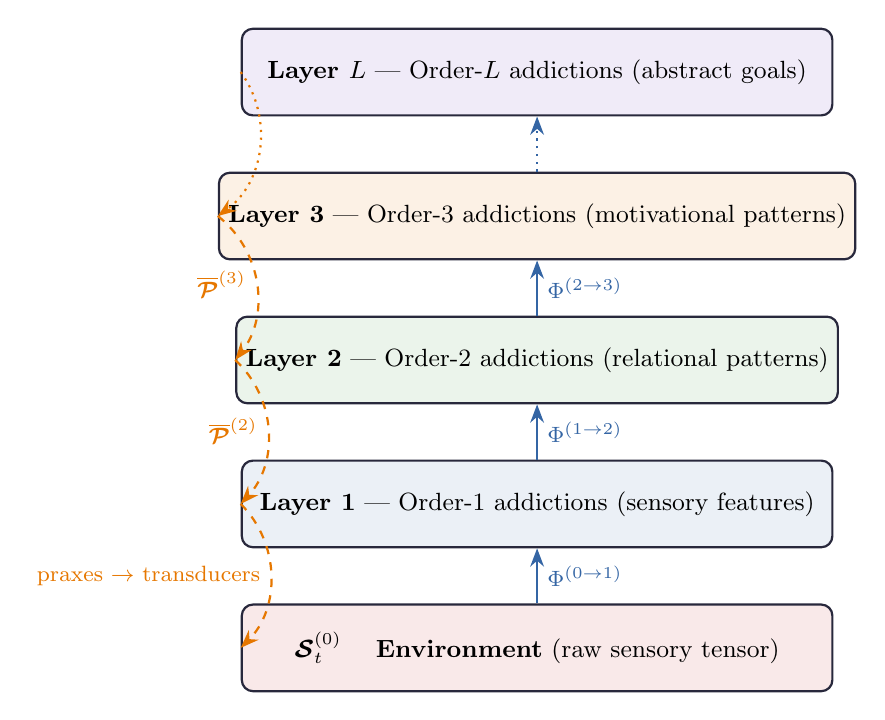
\begin{tikzpicture}[
  layer/.style={rectangle, rounded corners=4pt, draw=coldark, thick,
                minimum width=7.5cm, minimum height=1.1cm, fill=collight,
                font=\small},
  stim/.style={->, >=Stealth, thick, col1},
  prax/.style={->, >=Stealth, thick, col3, dashed},
  label/.style={font=\footnotesize, col1},
  plabel/.style={font=\footnotesize, col3},
  node distance=0.7cm
]
\node[layer, fill=col4!10] (L0)
    {$\tens{S}_t^{(0)}$ \quad \textbf{Environment} (raw sensory tensor)};
\node[layer, fill=col1!10, above=of L0] (L1)
    {\textbf{Layer 1} — Order-1 addictions (sensory features)};
\node[layer, fill=col2!10, above=of L1] (L2)
    {\textbf{Layer 2} — Order-2 addictions (relational patterns)};
\node[layer, fill=col3!10, above=of L2] (L3)
    {\textbf{Layer 3} — Order-3 addictions (motivational patterns)};
\node[layer, fill=col5!10, above=of L3] (LL)
    {\textbf{Layer $L$} — Order-$L$ addictions (abstract goals)};

% Stimulus upward arrows
\draw[stim] (L0.north) -- node[label,right]{$\Phi^{(0\to1)}$} (L1.south);
\draw[stim] (L1.north) -- node[label,right]{$\Phi^{(1\to2)}$} (L2.south);
\draw[stim] (L2.north) -- node[label,right]{$\Phi^{(2\to3)}$} (L3.south);
\draw[stim, dotted] (L3.north) -- (LL.south);

% Praxis downward (feedback) arrows on the left
\draw[prax] (L1.west) to[bend left=45]
    node[plabel,left]{praxes $\to$ transducers} (L0.west);
\draw[prax] (L2.west) to[bend left=45]
    node[plabel,left]{$\overline{\tens{P}}^{(2)}$} (L1.west);
\draw[prax] (L3.west) to[bend left=45]
    node[plabel,left]{$\overline{\tens{P}}^{(3)}$} (L2.west);
\draw[prax, dotted] (LL.west) to[bend left=45] (L3.west);
\end{tikzpicture}
\caption{The Addiction Emergence Ladder. Stimuli (solid blue arrows) propagate
upward through ILSC operators, increasing in abstraction. Praxes (dashed orange
arrows) propagate downward, modulating the stimulus construction at each level.
Each layer develops addictions of a higher order than the layer below.}
\label{fig:addiction_ladder}
\end{figure}

% ════════════════════════════════════════════════════════════
\section{Intricate Feedback Flows in ANN-$\Psi$}
\label{sec:feedback_flows}
% ════════════════════════════════════════════════════════════

\subsection{Three Classes of Feedback}

A running ANN-$\Psi$ exhibits not one but three structurally distinct classes of
feedback loop, which we now distinguish formally.

\paragraph{Class F1: Immediate Sensorimotor Loop.}
This is the basic AJN loop defined in Paper I: a unit at any layer emits praxes
$\tens{P}_t^{(j,\ell)}$, the transducers act on the environment, and the
environment returns a modified stimulus. The loop closes at time $t+1$:
\begin{equation}
\underbrace{\tens{S}_t^{(\ell)}}_{\text{stimulus}} \;\to\;
\underbrace{\tens{P}_t^{(j,\ell)}}_{\text{praxis}} \;\to\;
\underbrace{\mathcal{T}^{(\ell)}(\tens{P}_t^{(j,\ell)})}_{\text{transducer action}}
\;\to\; \underbrace{\tens{S}_{t+1}^{(\ell)}}_{\text{modified stimulus}}.
\label{eq:F1}
\end{equation}
The delay is one time step; the scope is local to the layer.

\paragraph{Class F2: Inter-Layer Modulatory Loop.}
The aggregate praxis of layer $\ell$ enters the ILSC operator and contributes to
the stimulus of layer $\ell+1$. But the craving levels of layer $\ell+1$ units
determine the addiction-weighted pooling in Eq.~\eqref{eq:pool} back at layer
$\ell$, completing a modulatory loop of scope $\pm 1$ layer:
\begin{equation}
\mathcal{M}^{(\ell+1)}(t)\; \xrightarrow{\text{weights } w_j^{(\ell)}} \;
\overline{\tens{P}}_t^{(\ell)} \;\xrightarrow{\Phi}\;
\tens{S}_t^{(\ell+1)} \;\to\;
\mathcal{M}^{(\ell+1)}(t+1).
\label{eq:F2}
\end{equation}
This loop operates at the inter-layer timescale and creates \textit{attentional
modulation}: deep-layer addiction states reshape what lower layers collectively
emphasize.

\paragraph{Class F3: Long-Range Resonance Loop.}
When the ANN-$\Psi$ is embedded in a physical environment, the deep-layer praxes
(which drive high-order transducers: locomotion, speech synthesis, complex
manipulation) modify the raw environmental tensor $\tens{S}_t^{(0)}$. This
modification propagates upward through all ILSC operators and eventually returns
to the deep layer that originally generated the praxis. The loop closes across
$L$ layers and an arbitrary number of environmental time steps:
\begin{equation}
\tens{P}_t^{(\ell,\text{deep})} \;\to\;
\Delta\tens{S}_{t+\Delta}^{(0)} \;\xrightarrow{\Phi^{(0\to1)}\circ\cdots\circ\Phi^{(L-1\to L)}}\;
\Delta\tens{S}_{t+\Delta}^{(L)} \;\to\;
\mathcal{M}^{(L)}(t+\Delta+1).
\label{eq:F3}
\end{equation}
The delay $\Delta \gg 1$ creates \textit{temporal credit assignment across the
full depth of the network}---the deep unit acts and waits many steps for the
consequence to reach it back through the hierarchy. This is the network
counterpart of long-horizon planning in reinforcement learning.

\subsection{Coupled Resonance Dynamics}

The three feedback classes coexist and interact. Let
$\mathbf{m}_t = [\mathcal{M}^{(j,\ell)}(t)]$ denote the full craving state vector
of all units. The joint dynamics obey a coupled map:
\begin{equation}
\mathbf{m}_{t+1} = \mathbf{G}\!\left(
\mathbf{m}_t,\,
\left\{\tens{S}_t^{(\ell)}\right\}_{\ell=0}^{L},\,
\left\{\tens{P}_t^{(j,\ell)}\right\}
\right),
\label{eq:coupled}
\end{equation}
where $\mathbf{G}$ is the global update operator composed of all F1, F2, F3
sub-functions. The fixed points of $\mathbf{G}$ (when they exist) correspond to
\textit{stable high-order addiction configurations}: states in which every layer's
craving is either saturated or in a steady withdrawal--reactivation cycle, and the
entire network is locked into a self-consistent goal-seeking attractor.

\begin{proposition}[Existence of High-Order Attractors]
\label{prop:attractor}
If the ILSC operators $\Phi^{(\ell\to\ell+1)}$ are Lipschitz-continuous with
constant $\Lambda_\ell$, and if the product
$\prod_{\ell=0}^{L-1} \Lambda_\ell < 1$ (contraction condition), then the
coupled map Eq.~\eqref{eq:coupled} admits at least one fixed point
$\mathbf{m}^* \in [0,1]^{\sum_\ell N_\ell}$, which is a stable
high-order addiction configuration.
\end{proposition}

The contraction condition is satisfied in practice when the transducers implement
saturating non-linearities (sigmoidal actuators, normalized motor commands), which
is the natural design for safe physical systems.

% ════════════════════════════════════════════════════════════
\section{The Tensorial Praxic Stream}
\label{sec:tps}
% ════════════════════════════════════════════════════════════

\subsection{Motivation: Why a Single Output Tensor Is Insufficient}

Classical neural networks treat output as an event: given input $x$, produce
$\hat{y}$ in a single forward pass. This model is adequate for static pattern
recognition but fails when:
\begin{enumerate}
\item The environment changes faster than the inference time of the full network;
\item The action space requires multiple sequential operations (e.g., a robotic
arm must grasp before it can lift);
\item Feedback from early actions is necessary to compute later actions correctly;
\item The ``output'' is inherently temporal (speech, music, a sequence of movements).
\end{enumerate}
An ANN-$\Psi$ operating in a real environment faces all four challenges
simultaneously. The appropriate model is the \textit{Tensorial Praxic Stream}.

\subsection{Formal Definition}

\begin{definition}[Tensorial Praxic Stream]
\label{def:tps}
A \emph{Tensorial Praxic Stream} (TPS) generated by ANN-$\Psi$ over a
time horizon $[t_0, t_0 + T]$ is a stochastic process
\[
\Pi = \left\{
\left(\tens{P}_{t_k},\; \tens{F}_{t_k},\; \tens{S}_{t_k}^{(0)}\right)
\right\}_{k=0}^{K},
\]
where:
\begin{itemize}
\item $\tens{P}_{t_k} \in \R^{m_k}$ is the \emph{partial praxis tensor}
emitted at time step $t_k$;
\item $\tens{F}_{t_k} = \mathcal{T}(\tens{P}_{t_k})$ is the transducer output
(physical action) at $t_k$;
\item $\tens{S}_{t_k}^{(0)}$ is the environmental state \emph{after} the
transducer action has taken effect, i.e., the feedback;
\item the emission times $t_0 < t_1 < \cdots < t_K$ are adapted to the process
(they may be random);
\item each $\tens{P}_{t_{k+1}}$ is a measurable function of
$\tens{S}_{t_0}^{(0)}, \ldots, \tens{S}_{t_k}^{(0)}$ (the causal structure).
\end{itemize}
\end{definition}

The key structural property of the TPS is its \textit{causal interleaving}: every
partial praxis depends on all preceding feedbacks. This distinguishes the TPS from
a simple sequence of independent actions.

\subsection{TPS Dynamics: The Closed-Loop Equation}

The TPS is generated by the following closed-loop recursion, which replaces the
single forward pass of classical networks:
\begin{equation}
\boxed{
\tens{P}_{t_{k+1}} = \Omega_{\text{net}}\!\left(
\mathcal{H}_{t_k},\;
\tens{S}_{t_k}^{(0)},\;
\mathbf{m}_{t_k}
\right)
}
\label{eq:tps_recursion}
\end{equation}
where $\Omega_{\text{net}}$ is the network-level policy (the composition of all
layer policies), $\mathcal{H}_{t_k}$ is the full history of stimuli and praxes
up to $t_k$, and $\mathbf{m}_{t_k}$ is the current craving state vector.

The environmental dynamics close the loop:
\begin{equation}
\tens{S}_{t_{k+1}}^{(0)} = \mathcal{E}\!\left(
\mathcal{T}(\tens{P}_{t_{k+1}}),\; \tens{S}_{t_k}^{(0)}
\right),
\label{eq:env_dynamics}
\end{equation}
where $\mathcal{E}$ is the environment transition operator (deterministic or
stochastic). Together, Eqs.~\eqref{eq:tps_recursion} and~\eqref{eq:env_dynamics}
define a \textit{stochastic recurrent dynamical system} over the joint state space
$(\tens{S}^{(0)}, \mathbf{m})$.

\subsection{TPS Dimensionality and Emission Rate}

An important design parameter is the \textit{emission schedule}: at what intervals
$\Delta t_k = t_{k+1} - t_k$ does the network emit partial praxes? Three
canonical regimes exist:

\begin{enumerate}
\item \textbf{Fixed-rate streaming} ($\Delta t_k = \Delta t$ constant): the
network emits a new praxis tensor at every $\Delta t$ time steps, regardless of
the feedback content. This is appropriate for real-time motor control where
regularity is required.

\item \textbf{Event-triggered streaming}: the network emits a new praxis tensor
only when the feedback tensor $\tens{S}_{t_k}^{(0)}$ changes by more than a
threshold $\epsilon$:
\begin{equation}
t_{k+1} = \min\!\left\{t > t_k \;:\;
\|\tens{S}_t^{(0)} - \tens{S}_{t_k}^{(0)}\|_F > \epsilon\right\}.
\label{eq:event_trigger}
\end{equation}
This conserves computational resources and is appropriate for sparse, high-impact
environmental changes.

\item \textbf{Addiction-driven streaming}: the emission schedule is modulated by
the craving state. A unit approaching saturation ($\alpha_t \to \alpha_{\max}$)
\textit{suppresses} its emission (Phase 3 in the AJN cycle), while a unit in
frustration (Phase 5) \textit{accelerates} its emission:
\begin{equation}
\Delta t_{k+1}^{(j)} = \Delta t_{\min} + (\Delta t_{\max} - \Delta t_{\min})
\cdot \frac{\alpha_{t_k}^{(j)}}{\alpha_{\max}}.
\label{eq:addict_rate}
\end{equation}
\end{enumerate}

\subsection{The TPS as a Generalization of Classical Output}

The classical single-shot output is recovered as a degenerate limit of the TPS:

\begin{proposition}[Classical Output as TPS Limit]
\label{prop:degenerate}
Let $K = 1$ (a single emission), $\rho = 0$ (no temporal memory in ILSC),
and $\Delta = 0$ (no delay in the long-range loop). Then the TPS
$\Pi = \{(\tens{P}_{t_0}, \tens{F}_{t_0}, \tens{S}_{t_1}^{(0)})\}$ reduces to
the single forward pass of a classical neural network:
$\hat{y} = f(x) \equiv \tens{F}_{t_0}$ where $x \equiv \tens{S}_{t_0}^{(0)}$.
\end{proposition}

This shows that the TPS is a strict generalization: every classical neural network
output is a TPS with $K=1$, but TPS with $K > 1$ and $\rho > 0$ encode
qualitatively richer input--output relationships.

\subsection{Information Flow in the TPS}

Define the \textit{TPS information tensor} at step $k$ as:
\begin{equation}
\mathcal{I}_{t_k} = \bigoplus_{s=0}^{k} \gamma^{k-s} \cdot
I\!\left(\tens{S}_{t_s}^{(0)}\right),
\label{eq:info_tensor}
\end{equation}
where $\gamma \in (0,1]$ is a temporal discount factor and $\oplus$ denotes
channel-wise accumulation. The TPS information tensor is a compressed history of
all past stimulus intensities, serving as a \textit{temporal context signal} that
modulates the generation of future partial praxes. When $\gamma = 1$ no past
information is discounted; when $\gamma \to 0$ only the most recent feedback
matters.

% ════════════════════════════════════════════════════════════
\section{Deep Agentic Flow: Synthesis}
\label{sec:daf}
% ════════════════════════════════════════════════════════════

\subsection{The DAF Framework}

We now synthesize the two contributions of this paper into a unified framework.

\begin{definition}[Deep Agentic Flow]
\label{def:daf}
A \emph{Deep Agentic Flow} (DAF) is the joint process:
\[
\text{DAF} = \left(
\text{ANN-}\Psi,\;
\left\{\Phi^{(\ell\to\ell+1)}\right\}_{\ell=0}^{L-1},\;
\Pi,\;
\mathcal{E}
\right),
\]
consisting of an ANN-$\Psi$ architecture, a stimulus hierarchy defined by ILSC
operators, a TPS $\Pi$ governing the output, and an environment $\mathcal{E}$.
DAF operates as a perpetual closed loop: the TPS acts on $\mathcal{E}$,
$\mathcal{E}$ returns stimuli that enter the bottom of the stimulus hierarchy,
the hierarchy propagates and transforms these stimuli upward, deep layers
develop and maintain high-order addictions, and the resulting network craving
state drives the next emission of partial praxes.
\end{definition}

\subsection{The DAF Computation Graph}

Figure~\ref{fig:daf_graph} presents the complete DAF computation graph, showing
the interplay of the three feedback classes with the stimulus hierarchy and TPS.

\begin{figure}[h!]
\centering
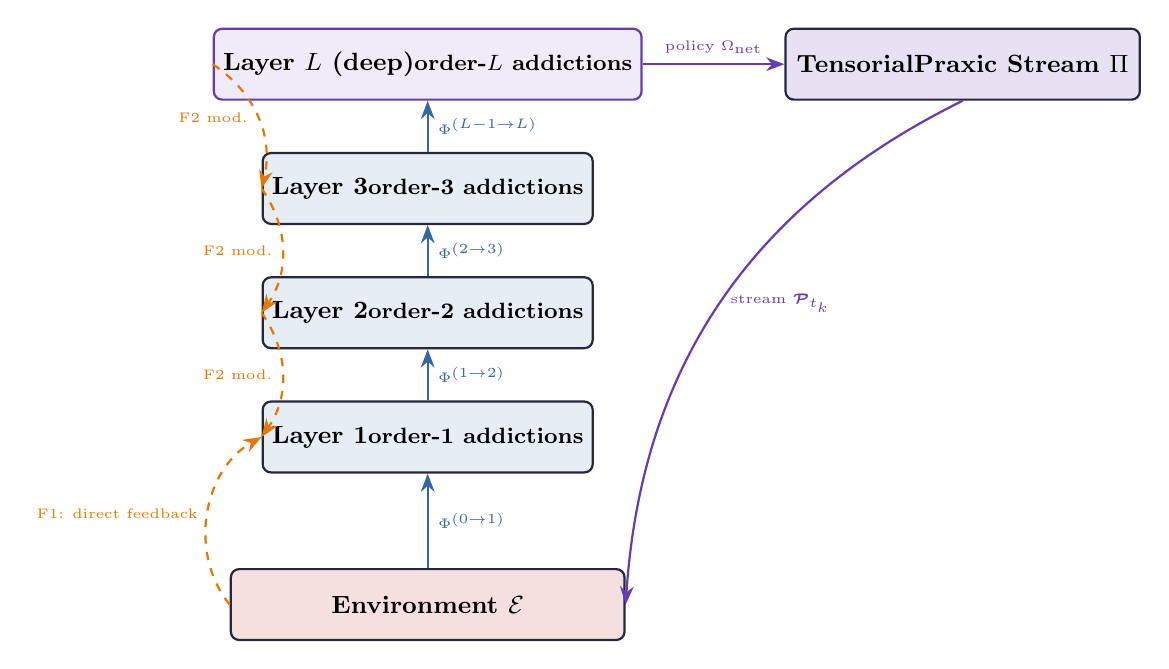
\begin{tikzpicture}[
  box/.style={rectangle, rounded corners=3pt, draw=coldark, thick,
              minimum width=3.2cm, minimum height=0.9cm, text centered,
              font=\small\bfseries},
  env/.style={box, fill=col4!15, minimum width=5cm},
  layer/.style={box, fill=col1!12},
  tps/.style={box, fill=col5!15, minimum width=4.5cm},
  arr/.style={->, >=Stealth, thick},
  farr/.style={->, >=Stealth, thick, col3, dashed},
  sarr/.style={->, >=Stealth, thick, col1},
  tarr/.style={->, >=Stealth, thick, col5},
  node distance=0.65cm and 1.5cm
]
% Environment
\node[env]  (env) {Environment $\mathcal{E}$};

% Layers bottom-up
\node[layer, above=1.2cm of env] (l1)
    {Layer 1 \\ {\footnotesize order-1 addictions}};
\node[layer, above=0.65cm of l1] (l2)
    {Layer 2 \\ {\footnotesize order-2 addictions}};
\node[layer, above=0.65cm of l2] (l3)
    {Layer 3 \\ {\footnotesize order-3 addictions}};
\node[layer, above=0.65cm of l3, draw=col5, fill=col5!10] (lL)
    {Layer $L$ (deep) \\ {\footnotesize order-$L$ addictions}};

% TPS block
\node[tps, right=1.8cm of lL] (tps)
    {Tensorial\\Praxic Stream $\Pi$};

% Stimulus upward arrows (F1 + ILSC)
\draw[sarr] (env.north) -- node[right, font=\tiny]{$\Phi^{(0\to1)}$}(l1.south);
\draw[sarr] (l1.north)  -- node[right, font=\tiny]{$\Phi^{(1\to2)}$}(l2.south);
\draw[sarr] (l2.north)  -- node[right, font=\tiny]{$\Phi^{(2\to3)}$}(l3.south);
\draw[sarr] (l3.north)  -- node[right, font=\tiny]{$\Phi^{(L-1\to L)}$}(lL.south);

% TPS output to environment (F3 long-range)
\draw[tarr] (tps.south) to[bend right=30]
    node[right, font=\tiny, col5]{stream $\tens{P}_{t_k}$} (env.east);

% Deep layer to TPS
\draw[tarr] (lL.east) -- node[above, font=\tiny, col5]{policy $\Omega_{\text{net}}$} (tps.west);

% Inter-layer modulatory feedback (F2)
\draw[farr] (l2.west) to[bend left=35]
    node[left, font=\tiny, col3]{F2 mod.} (l1.west);
\draw[farr] (l3.west) to[bend left=35]
    node[left, font=\tiny, col3]{F2 mod.} (l2.west);
\draw[farr] (lL.west) to[bend left=35]
    node[left, font=\tiny, col3]{F2 mod.} (l3.west);

% Env feedback back to layer 1 (F1 label)
\draw[farr] (env.west) to[bend left=50]
    node[left, font=\tiny, col3]{F1: direct feedback} (l1.west);
\end{tikzpicture}
\caption{The Deep Agentic Flow computation graph. Solid blue arrows: stimulus
propagation via ILSC operators. Dashed orange arrows: feedback flows (F1 direct,
F2 modulatory). Solid purple arrows: TPS emission and long-range loop (F3).
The deep layer drives the TPS, whose partial praxes act on the environment
and return as new stimuli at the bottom of the hierarchy.}
\label{fig:daf_graph}
\end{figure}

\subsection{DAF Algorithm}

\begin{algorithm}[H]
\caption{Deep Agentic Flow — Full Operational Cycle}
\begin{algorithmic}[1]
\STATE \textbf{Initialize:} ANN-$\Psi$ state $(\mathbf{m}_0, \tens{S}_0^{(0)},
       \{\boldsymbol{\mu}^{(j,\ell)}_0\})$; emission schedule; $k \leftarrow 0$
\WHILE{not terminated}
    % --- Upward stimulus propagation ---
    \FOR{$\ell = 1$ to $L$}
        \STATE Compute $w_j^{(\ell-1)} \leftarrow \softmax(\mathcal{M}^{(j,\ell-1)})$
        \STATE Pool: $\overline{\tens{P}}_{t_k}^{(\ell-1)}
               \leftarrow \sum_j w_j^{(\ell-1)} \tens{P}_{t_k}^{(j,\ell-1)}$
               \hfill \textit{// Eq.~\eqref{eq:pool}}
        \STATE Transduce: $\tens{F}_{t_k}^{(\ell-1)}
               \leftarrow \mathcal{T}^{(\ell-1)}(\overline{\tens{P}}_{t_k}^{(\ell-1)})$
        \STATE Construct: $\tens{S}_{t_k}^{(\ell)}
               \leftarrow (1-\rho)\tens{F}_{t_k}^{(\ell-1)}
               + \rho\,\tens{S}_{t_k-1}^{(\ell)}$
               \hfill \textit{// Eq.~\eqref{eq:memory}}
    \ENDFOR
    % --- Per-unit AJN update (all layers) ---
    \FOR{$\ell = 1$ to $L$, $j = 1$ to $N_\ell$}
        \STATE Run AJN cycle (Algorithm 1, Paper I) with input $\tens{S}_{t_k}^{(\ell)}$
        \STATE Update $\mathcal{M}^{(j,\ell)}$, $\theta^{(j,\ell)}$,
               $\boldsymbol{\mu}^{(j,\ell)}$, $\Sigma^{(j,\ell)}$
    \ENDFOR
    % --- TPS emission ---
    \STATE Determine emission time $t_{k+1}$ via chosen schedule
           (Eqs.~\eqref{eq:event_trigger} or~\eqref{eq:addict_rate})
    \STATE Compute $\tens{P}_{t_{k+1}} \leftarrow
           \Omega_{\text{net}}(\mathcal{H}_{t_k},
           \tens{S}_{t_k}^{(0)}, \mathbf{m}_{t_k})$
           \hfill \textit{// Eq.~\eqref{eq:tps_recursion}}
    % --- Environmental feedback ---
    \STATE Execute $\mathcal{T}(\tens{P}_{t_{k+1}})$ on $\mathcal{E}$
    \STATE Observe $\tens{S}_{t_{k+1}}^{(0)} \leftarrow
           \mathcal{E}(\mathcal{T}(\tens{P}_{t_{k+1}}), \tens{S}_{t_k}^{(0)})$
           \hfill \textit{// Eq.~\eqref{eq:env_dynamics}}
    % --- Long-range feedback (F3) ---
    \STATE Propagate $\tens{S}_{t_{k+1}}^{(0)}$ upward via ILSC operators
           (will take effect in next iteration)
    \STATE $k \leftarrow k+1$
\ENDWHILE
\end{algorithmic}
\end{algorithm}

\subsection{Emergent Temporal Structure of the TPS}

A DAF running under addiction-driven streaming (Eq.~\eqref{eq:addict_rate})
exhibits a characteristic temporal structure that reflects the collective
addiction state of the network:

\begin{itemize}
\item \textbf{Burst phases}: when the deep layer is in frustration (Phase 5),
$\Delta t_{k+1} \to \Delta t_{\min}$, and the TPS emits a rapid burst of
partial praxes---high-frequency, high-magnitude actions exploring the environment.
This corresponds to what an observer would describe as \textit{agitated,
searching behavior}.

\item \textbf{Quiescent phases}: when the deep layer is in saturation (Phase 3),
$\Delta t_{k+1} \to \Delta t_{\max}$, and the TPS emission slows dramatically.
The network acts minimally, maintaining its achieved state with low-energy
maintenance praxes. This corresponds to \textit{resting, satisfied behavior}.

\item \textbf{Rhythmic phases}: when the deep layer oscillates between withdrawal
and reinforcement (Phases 4 and 2), the emission rate oscillates accordingly,
producing a \textit{rhythmic, exploratory pattern}---periodic probing of the
environment with moderate-energy praxes.
\end{itemize}

These three behavioral modes emerge purely from the AJN addiction dynamics; no
external controller or scheduler is required.

% ════════════════════════════════════════════════════════════
\section{Discussion}
% ════════════════════════════════════════════════════════════

\subsection{High-Order Addictions and Cognitive Analogy}

The addiction emergence ladder (Section~\ref{sec:high_order}) has a provocative
interpretation when extended to many layers. An order-1 addiction is analogous
to a perceptual preference; an order-2 to a relational concept (``I crave the
co-occurrence of A and B''); an order-3 to a social or contextual expectation
(``I crave the state in which my subsystems are all satisfied simultaneously'').
At very deep layers, the addiction object becomes what one might loosely call a
\textit{value}: a stable internal attractor defined entirely in terms of the
network's own representational hierarchy.

This suggests that the Agentic Theory provides a \textit{bottom-up} account of
the emergence of abstract goals and values from simple low-level craving dynamics,
without requiring any top-down specification of what the system ``should'' want.

\subsection{TPS and Embodied Cognition}

The TPS formalization aligns with the enactivist and embodied cognition
traditions~\cite{varela1991embodied}, which argue that cognition is not input--output
mapping but a continuous, environmentally coupled process. The TPS makes this
precise: the network never ``finishes'' computing its output; it continuously
emits partial actions and absorbs partial feedbacks, with no clear boundary
between perception and action.

\subsection{Relation to Continuous Control and Recurrent Architectures}

The DAF framework can be seen as a principled extension of continuous-action
reinforcement learning and recurrent neural networks. Compared to LSTM- or
GRU-based architectures~\cite{hochreiter1997lstm}, the DAF temporal memory is
not stored in gated cell states but distributed across the craving levels of
all AJN units---a fundamentally different memory substrate. Compared to
policy gradient methods~\cite{williams1992reinforce}, the praxic policy update
operates locally at each unit and does not require a global advantage estimate.

\subsection{Open Problems}

\begin{enumerate}
\item \textbf{ILSC learning.} The ILSC operators $\Phi^{(\ell\to\ell+1)}$ are
currently fixed at design time. Learning them end-to-end---discovering what
transformations best support high-order addiction formation---is an open and
important problem.

\item \textbf{TPS truncation and horizon selection.} The DAF runs indefinitely;
real systems require principled criteria for truncating the TPS (``when is the
task done?''). Defining a network-level stopping condition in terms of
collective saturation is a natural direction.

\item \textbf{Multi-agent DAF.} If multiple ANN-$\Psi$ systems share the same
environment, their TPSs interact: one network's praxes modify the stimuli
available to the others. The emergent dynamics of multi-agent DAF---coalition,
competition, communication---constitute a rich and unexplored domain.

\item \textbf{Stability and controllability of high-order attractors.} While
Proposition~\ref{prop:attractor} guarantees the existence of attractors under
mild conditions, their stability margins, bifurcation structure, and
controllability (can we steer the network from one high-order addiction
configuration to another?) remain open questions.
\end{enumerate}

% ════════════════════════════════════════════════════════════
\section{Conclusion}
% ════════════════════════════════════════════════════════════

This paper has developed two foundational extensions to the Agentic Theory.

First, we showed that a stimulus tensor entering an AJN layer is not simply
consumed; it is \textit{transformed}, \textit{compressed or expanded}, and
\textit{passed upward} through a hierarchy of ILSC operators. Each level of the
hierarchy constructs a richer, more abstract stimulus space, enabling the
emergence of high-order addictions---stable craving attractors defined over
patterns that are purely internal products of the network's own dynamics and
have no direct sensory correlate. The addiction emergence ladder formalizes
this process and connects it to the three classes of feedback loop that
characterize a running ANN-$\Psi$.

Second, we argued that the output of an ANN-$\Psi$ is not a single tensor event
but a Tensorial Praxic Stream: a causally interleaved sequence of partial praxis
tensors, each conditioned on the environmental feedback from all preceding ones.
We defined the TPS formally, derived its closed-loop dynamics, characterized its
three canonical emission regimes, and showed that classical single-shot output is
a degenerate limit of the TPS.

Together, these two contributions define Deep Agentic Flow: a framework in which
the network's internal motivational hierarchy and its temporal behavioral stream
are co-constituted through the perpetual closed loop of action, feedback, and
recursive stimulus transformation. We believe DAF provides a principled new
language for describing adaptive, embodied, goal-directed artificial systems
whose goals are not programmed but \textit{grown}.

\section*{Acknowledgments}

This work builds on the AJN definition~\cite{tapiador2024ajn} and the
ANN-$\Psi$ architecture~\cite{tapiador2024annpsi}. The author acknowledges the
theoretical traditions of embodied cognition, free-energy minimization, and
intrinsically motivated reinforcement learning.

\begin{thebibliography}{99}

\bibitem{tapiador2024ajn}
Tapiador García, J. (2024).
Agentic Theory: Definition of the Artificial Junky Neuron (AJN).
\textit{Preprint, Universidad de Alicante}.

\bibitem{tapiador2024annpsi}
Tapiador García, J. (2024).
Agentic Theory II: The AJN and Its Integration into Multi-Layer Neural Architectures
(ANN-$\Psi$).
\textit{Preprint, Universidad de Alicante}.

\bibitem{sutton1998rl}
Sutton, R. S., \& Barto, A. G. (2018).
\textit{Reinforcement Learning: An Introduction} (2nd ed.).
MIT Press.

\bibitem{friston2010fep}
Friston, K. (2010).
The free-energy principle: a unified brain theory?
\textit{Nature Reviews Neuroscience}, 11(2), 127--138.

\bibitem{hochreiter1997lstm}
Hochreiter, S., \& Schmidhuber, J. (1997).
Long short-term memory.
\textit{Neural Computation}, 9(8), 1735--1780.

\bibitem{pathak2017curiosity}
Pathak, D., Agrawal, P., Efros, A. A., \& Darrell, T. (2017).
Curiosity-driven Exploration by Self-supervised Prediction.
\textit{Proceedings of ICML 2017}, 2778--2787.

\bibitem{varela1991embodied}
Varela, F. J., Thompson, E., \& Rosch, E. (1991).
\textit{The Embodied Mind: Cognitive Science and Human Experience}.
MIT Press.

\bibitem{williams1992reinforce}
Williams, R. J. (1992).
Simple statistical gradient-following algorithms for connectionist reinforcement
learning.
\textit{Machine Learning}, 8(3--4), 229--256.

\bibitem{lecun2015deep}
LeCun, Y., Bengio, Y., \& Hinton, G. (2015).
Deep learning.
\textit{Nature}, 521(7553), 436--444.

\bibitem{silver2016alphago}
Silver, D., et al. (2016).
Mastering the game of Go with deep neural networks and tree search.
\textit{Nature}, 529(7587), 484--489.

\bibitem{ha2018worldmodel}
Ha, D., \& Schmidhuber, J. (2018).
World Models.
\textit{arXiv preprint arXiv:1803.10122}.

\bibitem{oudeyer2007intrinsic}
Oudeyer, P.-Y., \& Kaplan, F. (2007).
What is intrinsic motivation? A typology of computational approaches.
\textit{Frontiers in Neurorobotics}, 1, 6.

\end{thebibliography}

\end{document}